\section{N-Queens problem with Las Vegas Approach}
\begin{frame}{What is the N-Queens Problem?}
  \begin{itemize}
    \item Place $N$ queens on an $N \times N$ chessboard so that no two queens threaten each other.
    \item Each queen must be in a different row, column, and diagonal.
    \item Number of possible arrangements grows rapidly with $N$ ($N!$ for rows/columns). \parencite{BELL20091}
  \end{itemize}
\end{frame}

\begin{frame}{Why is N-Queens Interesting?}
  \begin{itemize}
    \item \textbf{Computational Challenge:} Classic example of a constraint satisfaction problem. \parencite{motwani1995randomized}
    \item \textbf{Applications:}
          \begin{itemize}
            \item Constraint satisfaction problems
            \item Testing algorithms for search and optimization
            \item AI and backtracking benchmarks
          \end{itemize}
    \item \textbf{Why solve efficiently?} For large $N$, brute-force and naive methods become infeasible.
  \end{itemize}
\end{frame}

\begin{frame}[fragile]{How: Traditional Backtracking}
  \begin{itemize}
    \item Systematically tries to place queens row by row
    \item Backtracks when a conflict is detected
    \item \textbf{Time complexity:} $O(N!)$ in the worst case \parencite{motwani1995randomized}
  \end{itemize}
\end{frame}

\begin{frame}[fragile]{Traditional Backtracking: Pseudocode}
  \scriptsize
  \begin{algorithm}[H]
    \SetAlgoNlRelativeSize{-1}
    \SetKwFunction{FMain}{solve}
    \SetKwProg{Fn}{Function}{:}{}
    \Fn{\FMain{row}}{
      \If{row = N}{\Return true}
      \For{col $\leftarrow$ 0 \KwTo N-1}{
        \If{isSafe(row, col)}{
          placeQueen(row, col)\;
          \If{solve(row + 1)}{\Return true}
          removeQueen(row, col)\;
        }
      }
      \Return false
    }
  \end{algorithm}
\end{frame}

\begin{frame}{Why Consider Randomization?}
  \begin{itemize}
    \item Deterministic search (backtracking) can be slow for large $N$ \parencite{motwani1995randomized}
    \item Randomized (Las Vegas) algorithms can find solutions much faster on average \parencite{lasvegas1979babai}
    \item Demonstrates the power of probabilistic algorithms in combinatorial search
  \end{itemize}
\end{frame}

\begin{frame}{How: Las Vegas (Randomized) Approach}
  \begin{itemize}
    \item For each row, randomly select a safe column
    \item If stuck (no safe columns), restart from scratch
    \item Always finds a correct solution (if one exists), but runtime is random
    \item \textbf{Expected time:} Much faster than backtracking for large $N$ \parencite{lasvegas1979babai}
  \end{itemize}
\end{frame}

\begin{frame}[fragile]{Las Vegas (Randomized) Approach: Pseudocode}
  \scriptsize
  \begin{algorithm}[H]
    \SetAlgoNlRelativeSize{-1}
    \SetKwFunction{FMain}{lasVegasNQueens}
    \SetKwProg{Fn}{Function}{:}{}
    \Fn{\FMain{N, maxAttempts}}{
      \For{attempt $\leftarrow$ 1 \KwTo maxAttempts}{
        board $\leftarrow$ empty\_board(N)
        success $\leftarrow$ true
        \For{row $\leftarrow$ 0 \KwTo N-1}{
          safeCols $\leftarrow$ get\_safe\_columns(row, board)
          \If{safeCols is empty}{success $\leftarrow$ false; \textbf{break}}
          col $\leftarrow$ random choice from safeCols
          place\_queen(row, col, board)
        }
        \If{success}{\Return board}
      }
      \Return None
    }
  \end{algorithm}
\end{frame}

\begin{frame}{Performance Comparison (Visualization)}
  \vfill
  \begin{center}
    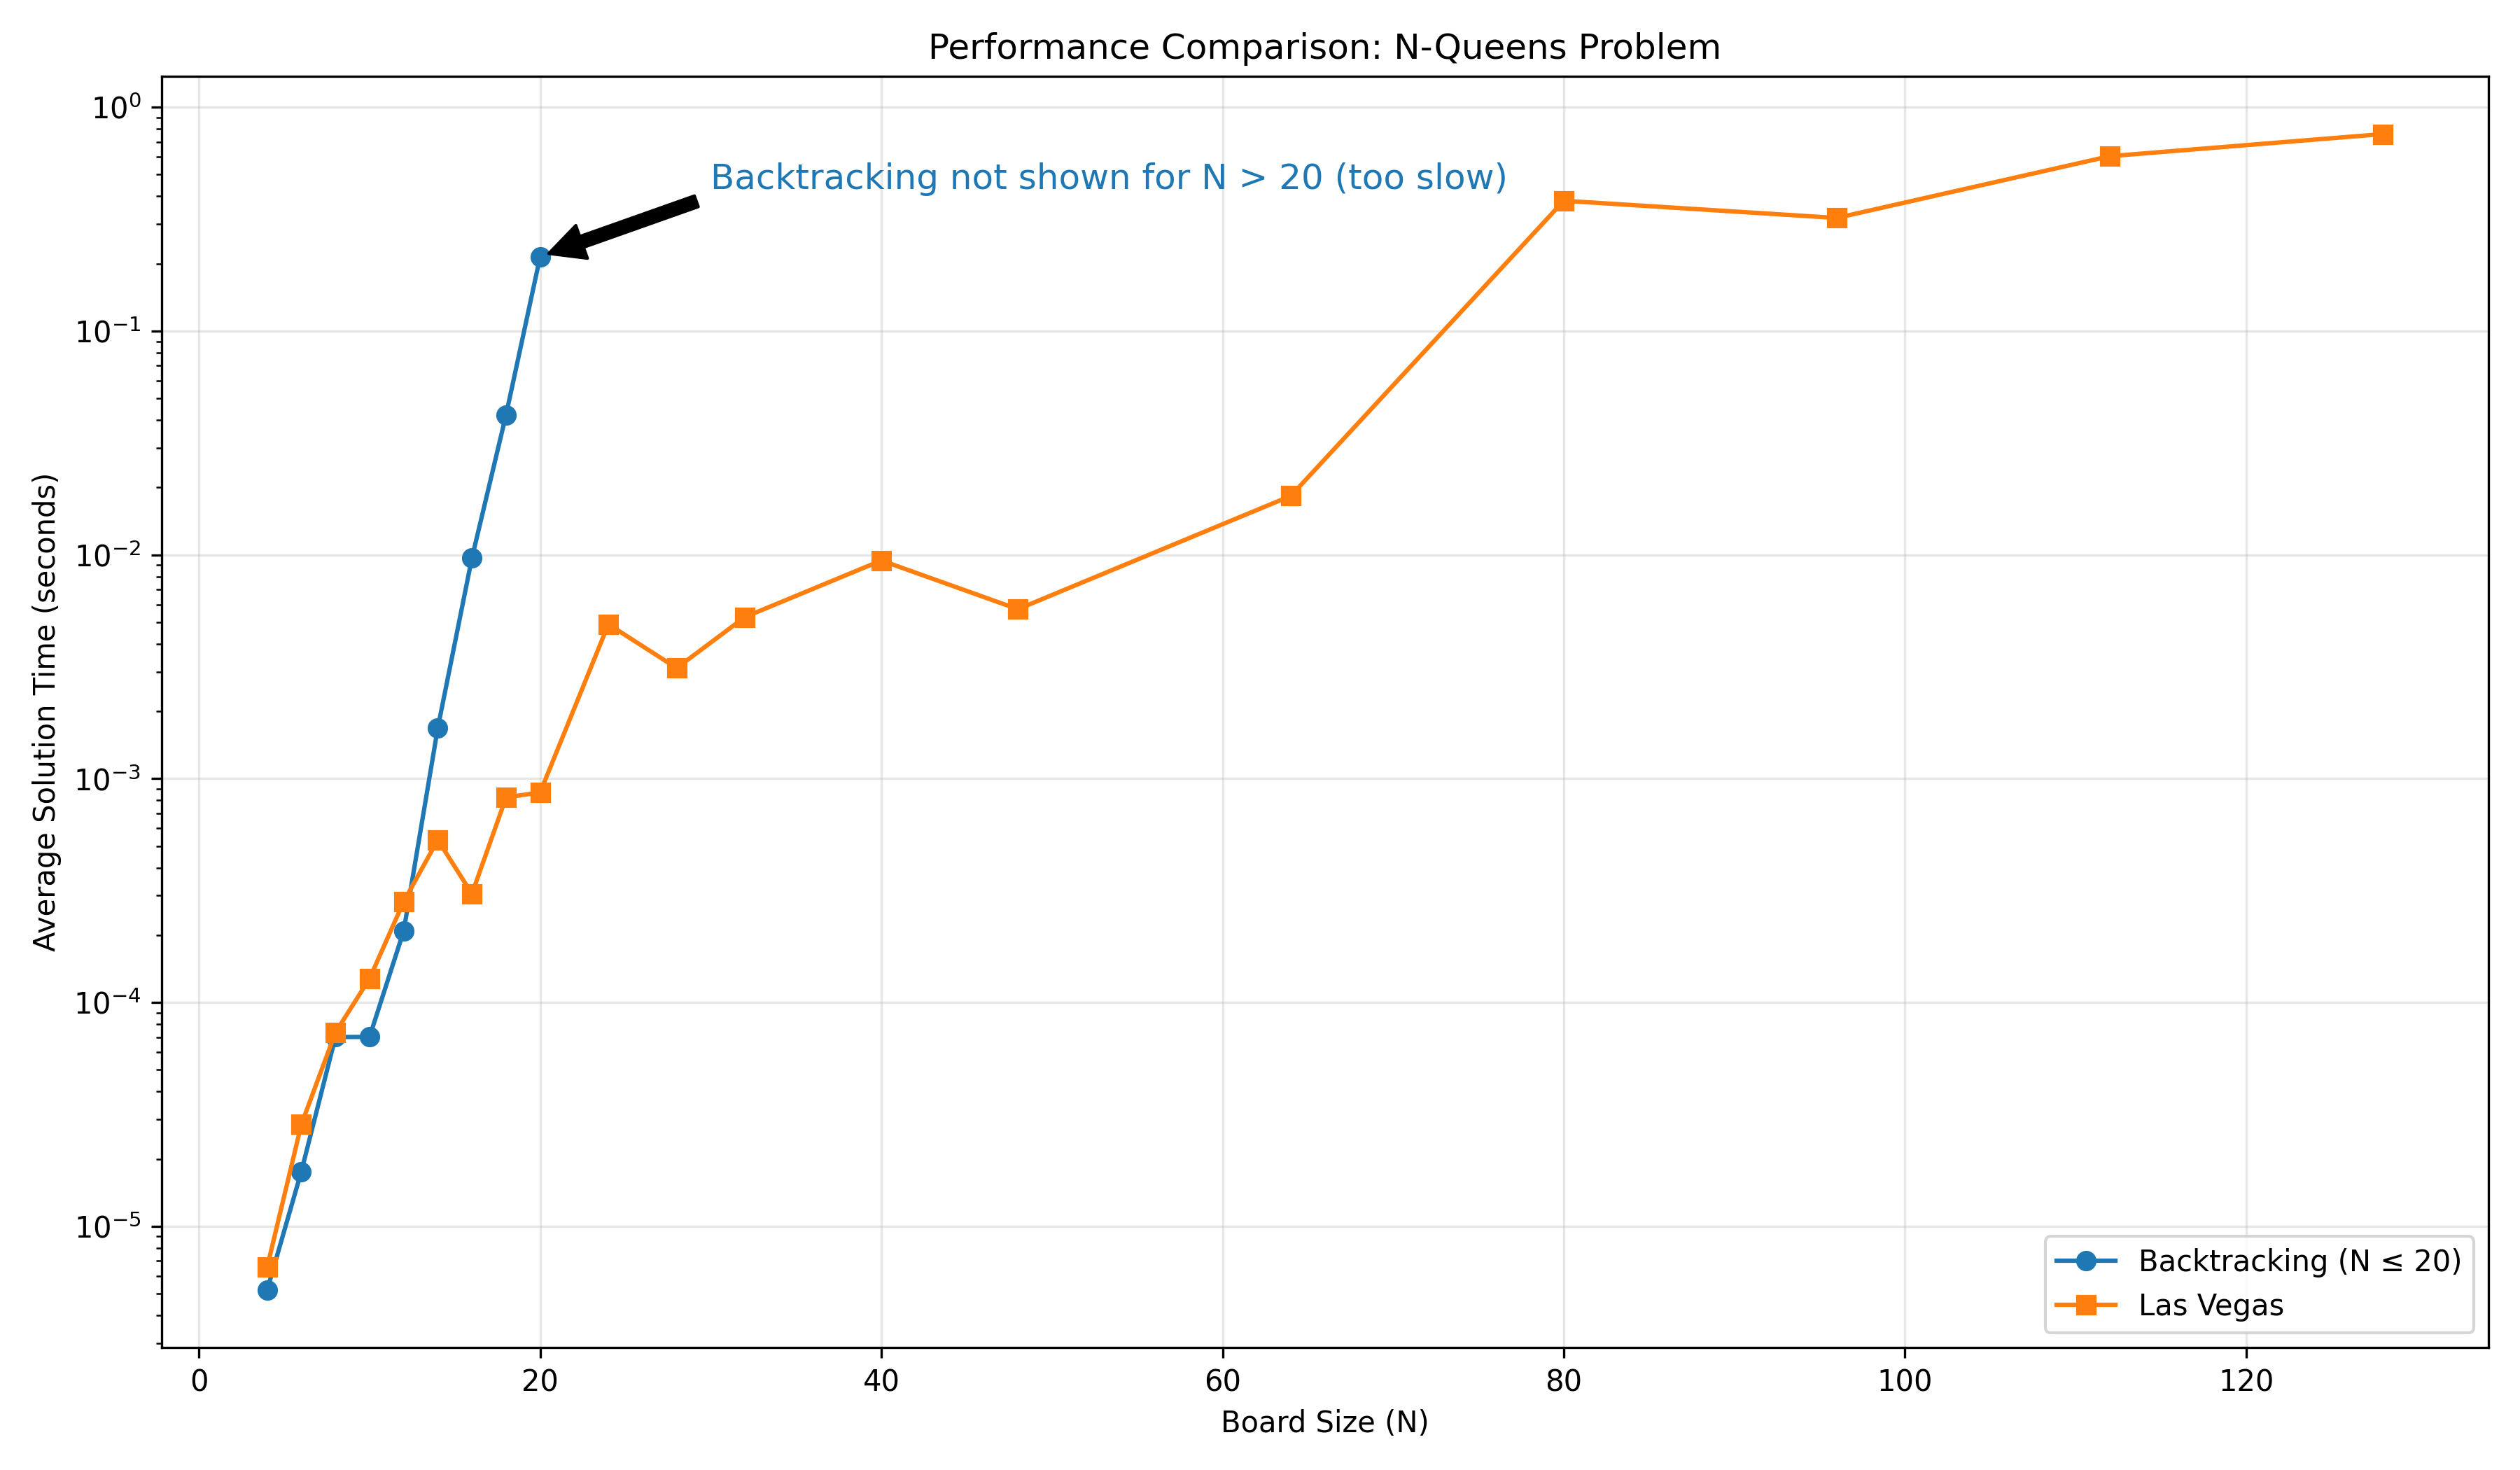
\includegraphics[height=0.95\textheight]{./programs/nqueens-lv/images/performance-comparison.png}
  \end{center}
  \vfill
\end{frame}

\begin{frame}{Performance Comparison (Interpretation)}
  \begin{itemize}
    \item Average solution time vs. $N$ for Backtracking and Las Vegas approaches.
    \item Las Vegas (randomized) is much faster for large $N$.
    \item Backtracking becomes infeasible as $N$ grows.
  \end{itemize}
\end{frame}

\begin{frame}{Performance Comparison}
  \begin{itemize}
    \item \textbf{Backtracking:}
          \begin{itemize}
            \item Deterministic, exhaustive search
            \item Predictable but slow for large $N$
          \end{itemize}
    \item \textbf{Las Vegas:}
          \begin{itemize}
            \item Randomized, may restart
            \item Runtime varies, but much faster on average for large $N$
          \end{itemize}
  \end{itemize}
\end{frame}

\begin{frame}{Key Insights}
  \begin{itemize}
    \item Randomization can dramatically improve performance for some combinatorial problems \parencite{motwani1995randomized}
    \item Las Vegas algorithms always produce correct results, but runtime is a random variable \parencite{lasvegas1979babai}
    \item For N-Queens, Las Vegas approach is practical for very large $N$ where backtracking is infeasible
    \item Illustrates the power of probabilistic algorithms in search and optimization
  \end{itemize}
\end{frame}